Toy operators check the measure where the answer is known in advance. We combine two Gaussian parts in $\R^{16}$ by fourteen operators, from role--filler binding (concatenation and a tensor product) through fixed-width superposition (random projections into $0.5$ to $1.5$ times $kd = 32$ dimensions, HRR and multiply--add--permute (MAP) binding \citep{plate1995,gayler2006,kanerva2009}, and $x + 0.5y$) to symmetric blends ($x + y$ and $x \odot y$) and a random $\tanh$ layer. We fit ridge, least-squares and MLP probes of the role-1 part on wholes built from a vocabulary of $V$ parts, with 5 seeds for each $V$.

\begin{figure}[t]
  \centering
  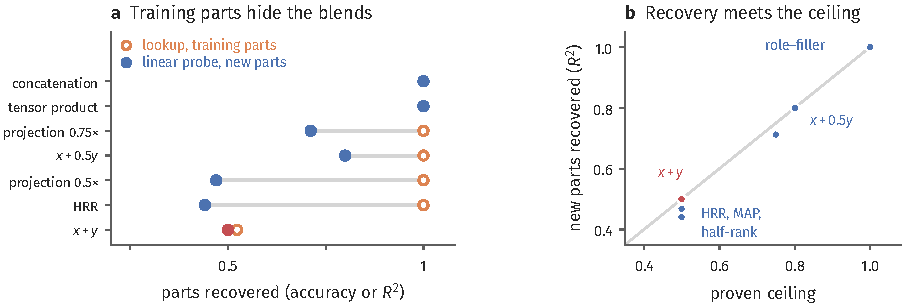
\includegraphics[width=\linewidth]{fig_measure.pdf}
  \caption{\textbf{Training parts hide blends, and new parts expose them.} \textbf{a.} A lookup over wholes built from 32 training parts (open orange) identifies the role-1 part of every operator except the symmetric blend, while a linear probe separates the operators on new parts (filled; red marks $x + y$). \textbf{b.} Linear recovery of new parts meets the ceiling of Proposition~\ref{prop:ceiling}. Means over 5 seeds.}
  \label{fig:measure}
\end{figure}

A lookup identifies the role-1 part of every operator that keeps the vocabulary distinct with accuracy 1.00, including half-rank projections and HRR, which keep only half of each part, and fails only on the symmetric blends, at 0.52 (Figure~\ref{fig:measure}a). A test on training parts therefore confuses role--filler binding with vector-symbolic superposition. At $V = 128$, linear probes recover the role--filler operators and full-rank projections at $R^2 = 1.00$, half-rank projections at 0.47 and $x + 0.5y$ at 0.80, its ceiling (Figure~\ref{fig:measure}b). HRR and MAP reach 0.44 and 0.47, close to their common ceiling of $1/2$. Flexible probes do worse because they memorize the vocabulary, and an MLP probe recovers only 0.11 of the half-rank projection on new parts, so every later test fixes a linear probe in advance.
